\section{Resultados}

No presente capítulo, são apresentados os resultados obtidos, a partir da observação do funcionamento do protótipo construído. Serão apresentados imagens demonstrando o funcionamento e além disso serão destacados os desafios enfrentados durante o processo e as estratégias adotadas para mitigá-los.

\subsection{Resultados}

Ao implementar o protocolo \textit{start-stop} o primeiro resultado obtido foram caracteres recebidos diferentes do enviado. A causa do erro foi o tempo de leitura do receptor que ao ler o código de start, que é representado pelo byte 11111110, o último bit estava sendo considerado como parte da mensagem.

\begin{figure}[!htbp]
  \caption{As informações mostradas pelo emissor e receptor não correspondem}
  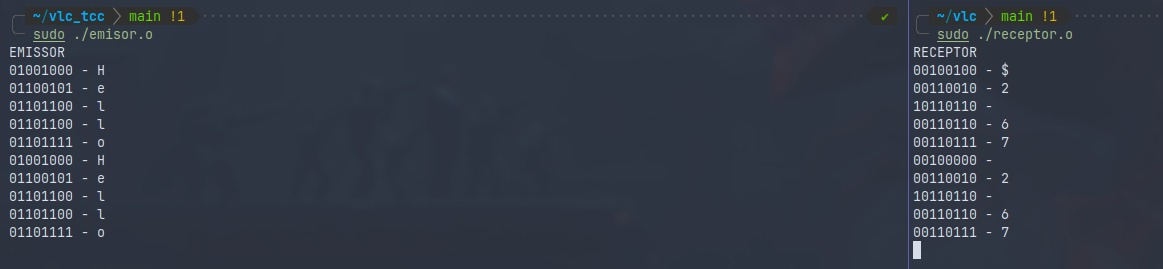
\includegraphics[width=0.9\textwidth]{images/vlc_erro_1.jpeg}
  \legend{Fonte: Autor (2023)}
  \label{primeiro_erro}
\end{figure}

\begin{figure}[!htbp]
  \caption{Comparação entre os bytes enviados e recebidos}
  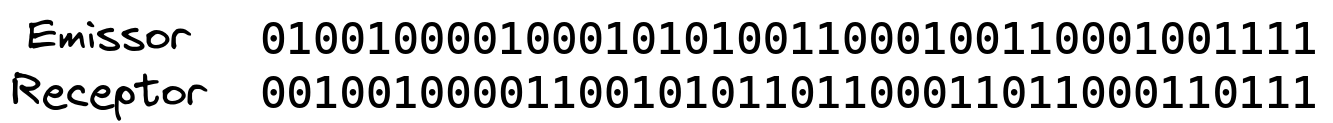
\includegraphics[width=0.9\textwidth]{images/comparacao_msg_emissor_recptor_erro.png}
  \legend{Fonte: Autor (2023)}
  \label{comparaca_msg_emissor_recptor_erro}
\end{figure}

Após a correção do problema de temporização, os cinco bytes são enviados sem erros. A taxa de transmissão atingida foi de 10 bits por segundo. Não foi viável aumentar a taxa devido às limitações da \textit{Single Board Computer} (SBC), que não suporta leituras mais rápidas, e também devido ao tempo de resposta desfavorável do circuito com o ldr.

\begin{figure}[!htbp]
  \caption{Transmissão correta da mensagem}
  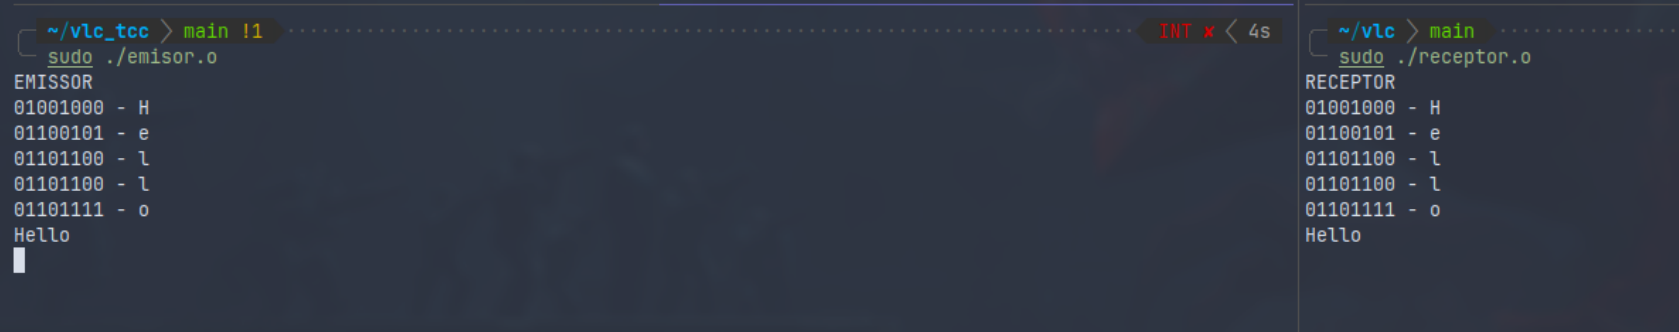
\includegraphics[width=0.8\textwidth]{images/vlc_run.png}
  \legend{Fonte: Autor (2023)}
  \label{vlc_funcionando}
\end{figure}

\begin{figure}[!htbp]
  \caption{Foto do prototipo funcionando}
  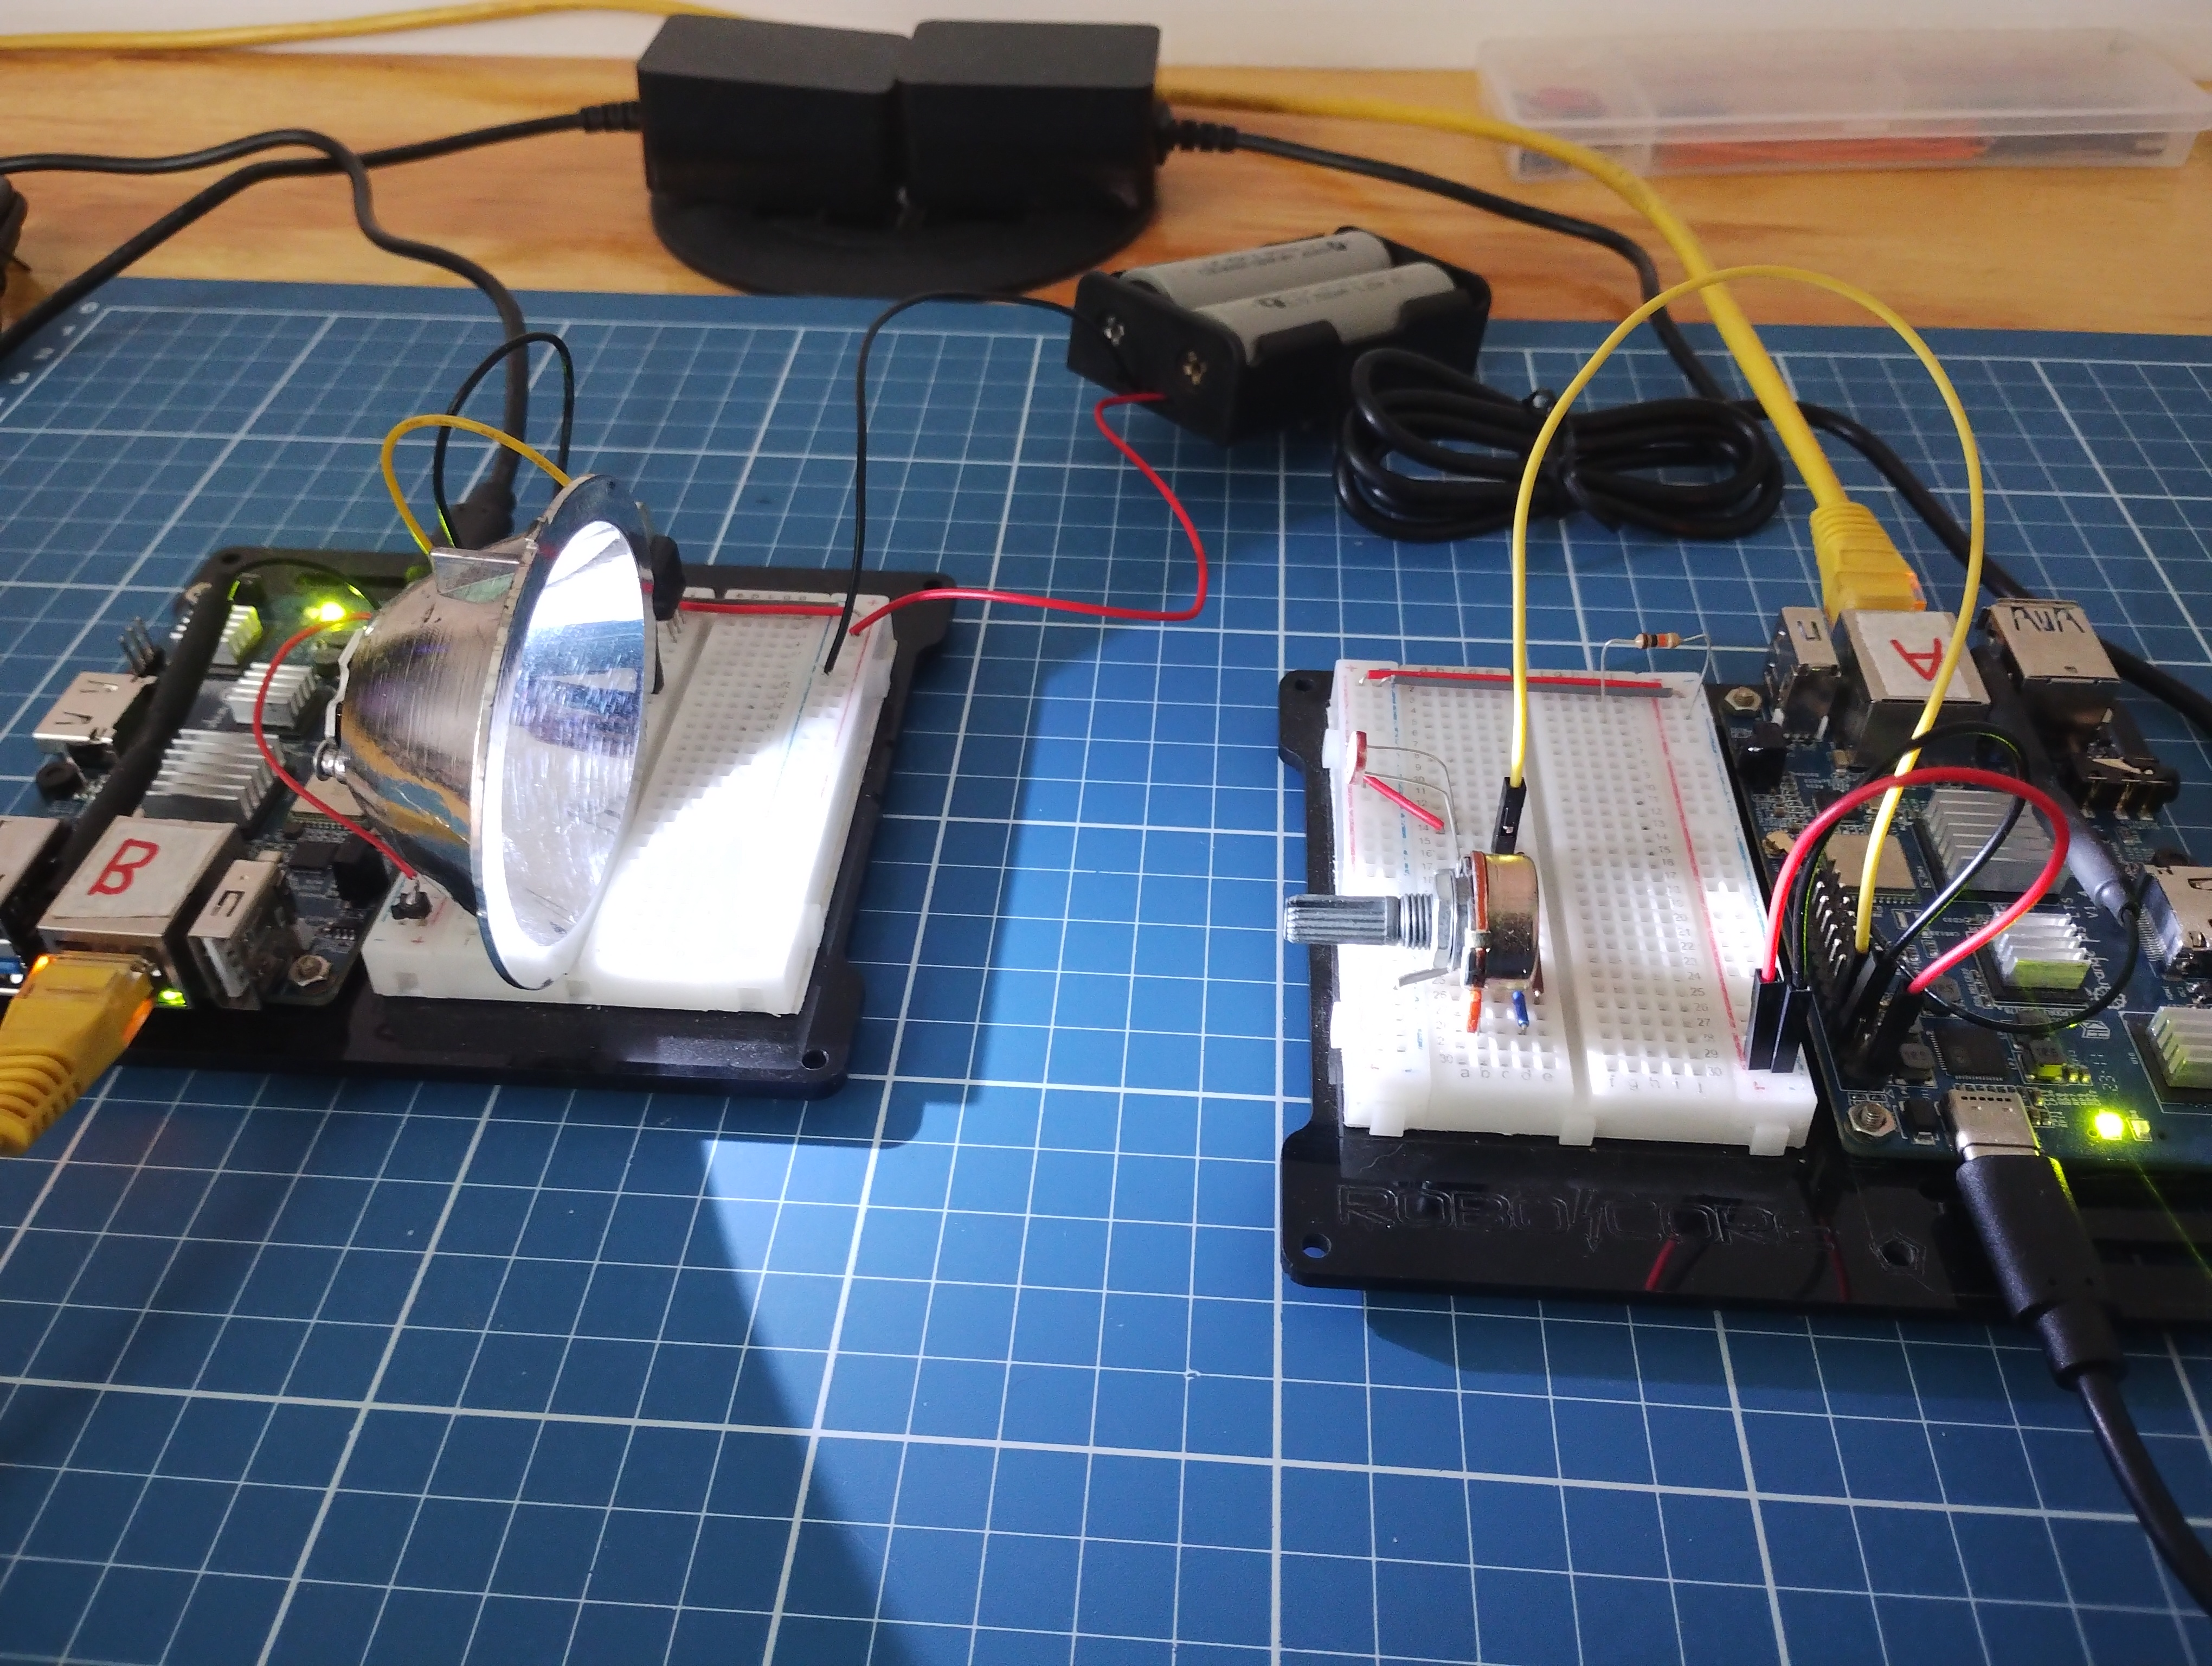
\includegraphics[width=0.6\textwidth]{images/vlc_funcionamento.jpg}
  \legend{Fonte: Autor (2023)}
  \label{vlc_funcionando_foto}
\end{figure}


\subsection{Dificuldades}

Durante o desenvolvimento do protótipo encontrou-se diversos pontos de dificuldade. Dentre eles está o fato do projeto da SBC \textit{OrangePi} não ser muito maduro, resultando em pouca documentação para a biblioteca \textit{wiringOP}, responsável por manipular as GPIOs.

Outro ponto é o fato da SCB não possuir um conversor analógico-digital (ADC), sendo necessário montar um circuito para isso. A solução utilizada foi uma muito simples, um potenciômetro ligado em série com um ldr, mas permite estabelecer uma faixa de corte e a leitura de se está claro ou escuro, ou em outras palavras se é 1 ou 0.

